\documentclass[24pt,margin=1in,innermargin=-7in,blockverticalspace=-0.25in]{tikzposter}
\geometry{paperwidth=47.24in,paperheight=35.43in}
\usepackage[utf8]{inputenc}
\usepackage{amsfonts}
\usepackage{amssymb}
\usepackage{mathrsfs}
\usepackage{graphicx}
\usepackage{adjustbox}
\usepackage{enumitem}
\usepackage[backend=biber,style=numeric]{biblatex}
\usepackage{uomtheme}
\usepackage{booktabs, amsthm, amsmath}
\usepackage{caption}
\usepackage{tikz}
\usetikzlibrary{arrows, automata, positioning}


\usepackage{mwe} % for placeholder images

\addbibresource{refs.bib}

% set theme parameters
\tikzposterlatexaffectionproofoff
\usetheme{UoMTheme}
\usecolorstyle{UoMStyle}

\usepackage[scaled]{helvet}
\renewcommand\familydefault{\sfdefault} 
\usepackage[T1]{fontenc}

\title{Diffusion for Offline Bandit}
\author{Shouchen Zhou, Xinyue Ying}
% \author{%
%   Shouchen Zhou\\
%     \texttt{zhou.sc@shanghaitech.edu.cn}\\
%   Xinyue Ying\\
%   \texttt{yingxy@shanghaitech.edu.cn}
% }
\institute{ShanghaiTech University}

% \titlegraphic{
\includegraphics[width=0.06\textwidth]{Img/Shanghaitch_logo.png}}
% \titlegraphic{
\includegraphics[width=0.06\textwidth]{Img/ShanghaiTech.png}}

\newcommand{\x}{\mathbf{x}}


\makeatletter
\setlength{\TP@titlegraphictotitledistance}{0cm} 
% remove default spacing if needed
\settitle{
  \begin{tikzpicture}[remember picture,overlay]
    \node[anchor=north west, xshift=-35cm, yshift=-1cm] at (current page.north west)
      {
\includegraphics[width=0.17\textwidth]{Img/ShanghaiTech.png}};

    \node[anchor=north west, xshift=40cm, yshift=-1.2cm] at (current page.north west)
      {
\includegraphics[width=0.05\textwidth]{Img/Shanghaitch_logo.png}};
  \end{tikzpicture}
  \centering
  \color{titlefgcolor}
  {\bfseries \Huge \sc \@title \par}
  \vspace{0.5em}
  {\huge \@author}
}
\makeatother


% begin document
\begin{document}
\maketitle
\centering
\begin{columns}
    \column{0.32}
    \block{Introduction}
    {
        \textbf{Diffusion models}\cite{campbell2022continuous} are generative models that learn data distributions through step-by-step denoising. While popular in image generation, they also excel at modeling complex, multimodal structures in other domains.

\begin{center}
    \begin{tikzpicture}[->, >=stealth, auto, thick, node distance=1.5cm]
        \tikzstyle{every state} = [
            fill=gray!30,
            draw=black,
            circle,
            minimum size=40pt,
            font=\large\bfseries
        ]

        \tikzstyle{ellipsis state} = [
            fill=none,
            draw=none,
            circle,
            minimum size=20pt
        ]

        \node[state] (1) {$\x_T$};
        \node[ellipsis state] (ellipsis1) at (4,0) {$\cdots$};
        \node[state] (2) at (8, 0) {$\x_t$};
        \node[state] (3) at (16, 0) {$\x_{t-1}$};
        \node[ellipsis state] (ellipsis2) at (20, 0) {$\cdots$};
        \node[state] (4) at (24, 0) {$\x_0$};

        \draw[->] (1) -- (ellipsis1);
        \draw[->] (ellipsis1) -- (2);

        \draw[->] (2) -- (3) node[midway, above] {$p_{\theta}(\x_{t-1}|\x_t)$};

        \path (3) edge[bend left=30, dashed] node[midway, below] {$q(\x_t|\x_{t-1})$} (2);

        \draw[->] (3) -- (ellipsis2);
        \draw[->] (ellipsis2) -- (4);
    \end{tikzpicture}
    \captionof{figure}{Diffusion model represented as a Markov chain, with a forward process for noise addition during training and a backward process for denoising and generation.}
\end{center}

In this work, we explore diffusion in \textbf{offline bandit learning} from two perspectives:

\begin{itemize}
     \item \textbf{Stochastic Bandit}: A discrete diffusion model generates additional trajectories from interaction logs, expanding the limited offline dataset to enhance pretraining and reduce exploration costs.

    \item \textbf{Contextual Bandit}: A diffusion model is trained to approximate the conditional reward distribution \( P(r \mid c, a) \), enabling action selection via sampling and capturing aleatoric uncertainty.
\end{itemize}
    }
    
    \block{Stochastic Bandit}
    {
        \begin{itemize}
    \item Traditional algorithms: cold start or rely on limited offline logs, which suffer from size limitations, narrow coverage, and distribution bias, constraining performance.
    \item Our approach: employ a discrete diffusion model to synthesize additional pseudo-trajectories, broadening data diversity and coverage, and apply a policy gradient based bandit algorithm to fully exploit the expanded offline dataset.
\end{itemize}

Similarly to the policy gradient methods~\cite{sutton1999policy} in Reinforcement Learning algorithms, in the bandit settings, the online interaction log of a stochastic multi-armed bandit can be viewed as a trajectory composed of action–reward pairs.
\begin{equation}
\psi=\left(a_0,r_1,\cdots,,a_{T-1},r_T\right).
\end{equation}
By archiving several past trajectories into an offline dataset, we can pre-train the stochastic bandit and thereby cut down the cost of subsequent online interactions. The probability of encountering a specific trajectory $\psi$ is
\begin{equation}
P_{\theta}(\psi)=\prod_{t=0}^{T-1}\pi_{\theta}(a_t \mid a_0, r_1,\ldots, a_{t-1},r_t).
\end{equation}
The objective function is given by
\begin{equation}
J(\theta) = \mathbb{E}_{\Psi\sim P_{\theta}}\left[R(\Psi)\right] = \sum_{\psi}P_{\theta}(\psi)R(\psi).
\end{equation}
The policy gradient can be expressed as
\begin{equation}
\nabla_{\theta}J(\theta) \approx \dfrac{1}{m}\sum_{i=1}^m\sum_{t=0}^{T-1}\left[\left(R_t^i - b_t\right) \nabla_{\theta}\log\pi_{\theta}\left(a_t^i \mid a_0^i, r_1^i,\ldots, a_{t-1}^i,r_t^i\right)\right] \\
\end{equation}
Thus, given an offline dataset, we improve stochastic bandit performance:

1. \textbf{Dataset expansion}: generate extra trajectories with diffusion model.

2. \textbf{Pre-training}: train stochastic bandit algorithms on the enlarged dataset.

3. \textbf{Online adaptation}: run and refine the pretrained agents online.

With the pretrained weights, the policy executed at each online step is:
\begin{equation}
\pi_{\theta}(a)=\dfrac{e^{\beta_tH_{\theta}(a)}}{\sum_{a'} e^{\beta_tH_{\theta}(a')}}
\end{equation}
Which is similar to the traditional gradient bandit algorithm~\cite{gradient_bandit}, and has similar online update rules. 
The non-Bernoulli distribution $X \in \{0,\,0.5,\,1\}$ with probs $\theta_1,\theta_2,1-\theta_1-\theta_2$ was also used to test the performance.
    }
    

    \column{0.36}

    \block{Contextual Bandit}
    {
        \begin{itemize}
    \item Traditional algorithms: estimating the expected reward and epistemic uncertainty. 
    \item In real-world scenarios, distributional features such as multimodality, skewness, and heavy tails, reflecting aleatoric uncertainty, can provide valuable information for decision-making.
\end{itemize}
    \begin{minipage}[t]{0.45\linewidth}
    \vspace{10pt} % 强制顶部对齐
    This project investigates a method that makes decisions by directly sampling from the full conditional reward distribution $P(r \mid c, a)$, which is learned through a diffusion model.
    \end{minipage}
\hfill
\begin{minipage}[t]{0.48\linewidth}
\vspace{0pt}
    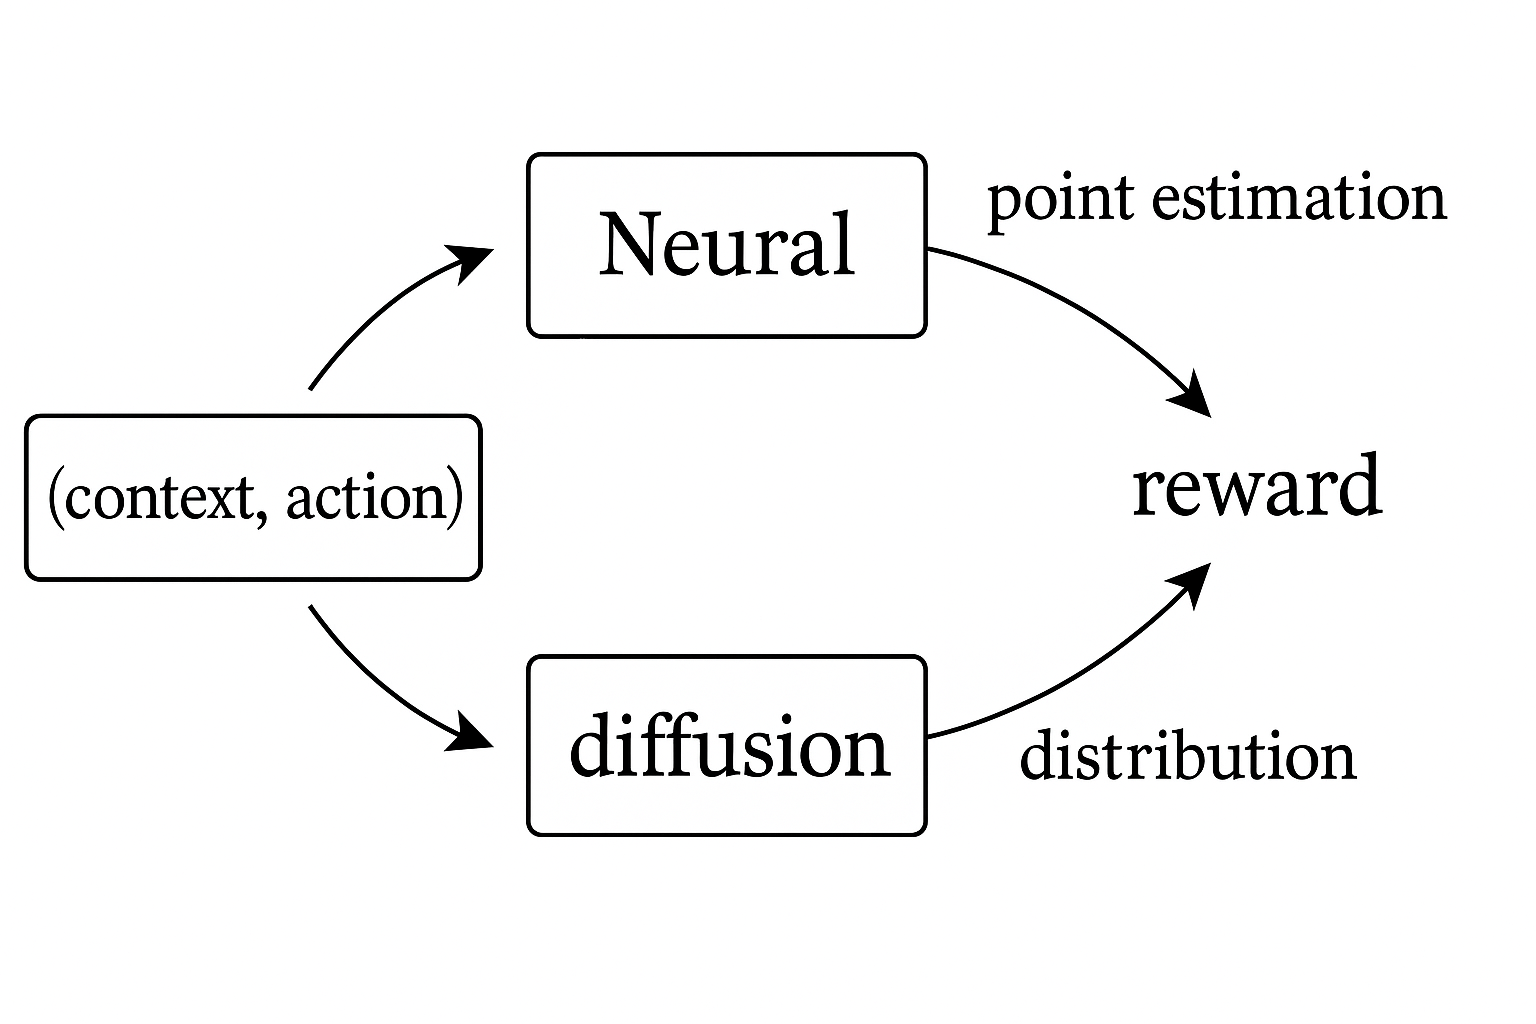
\includegraphics[width=\linewidth]{Img/context_diffusion.png}
\end{minipage}
\textbf{Reward Distribution Modeling:}

Pretrain: A diffusion model is trained on $(c, a, r)$ data to approximate $P(r \mid c, a)$.

\textbf{Action Selection (at context $c_t$):}
\begin{enumerate}
    \item For each action $a$: sample $\tilde{r}_a \sim P(r \mid c_t, a; W_{\text{diffusion}})$ using the trained diffusion model.
    \item Choose action: $a_t = \arg\max\limits_{a \in \mathcal{A}} \tilde{r}_a$.
\end{enumerate}
    }
    
    \block{Stochastic Bandit Results}
    {
        \begin{center}
    % \vspace{-0.2in}
\begin{tabular}{cccc}
  \toprule
  Trajectory generation policy & UCB & TS & policy gradient \\
  \midrule
  no offline dataset                           & 1691.827 & 163.483 & 858.794 \\
  offline, no enlarge                          & 1303.405 &  43.550 &  82.254 \\
  offline+copy                                 & 1156.635 &  26.596 &  54.048 \\
  offline+diffuse pair                         & 1028.613 &   7.296 &  42.993 \\
  offline+diffusion sequence                   &  923.779 &   0.071 &   3.522 \\
  offline+diffusion sequence (Transformer)     &  743.441 &   0.008 &   0.002 \\
  \bottomrule
\end{tabular}
    \captionof{table}{Performance(average accumulated regret) of various algorithms on Bernoulli-reward bandits under different offline-dataset enlargement (trajectory-generation) policies.}
    % \vspace{-0.45in}
\end{center}


\begin{tikzfigure}[Performance of each algorithm(UCB, policy gradient) across arm counts(20, 25, 30) with non-Bernoulli rewards, evaluated under three pre-training settings: none, offline (500 trajectories generated by diffusion sequence (Transformer).]
    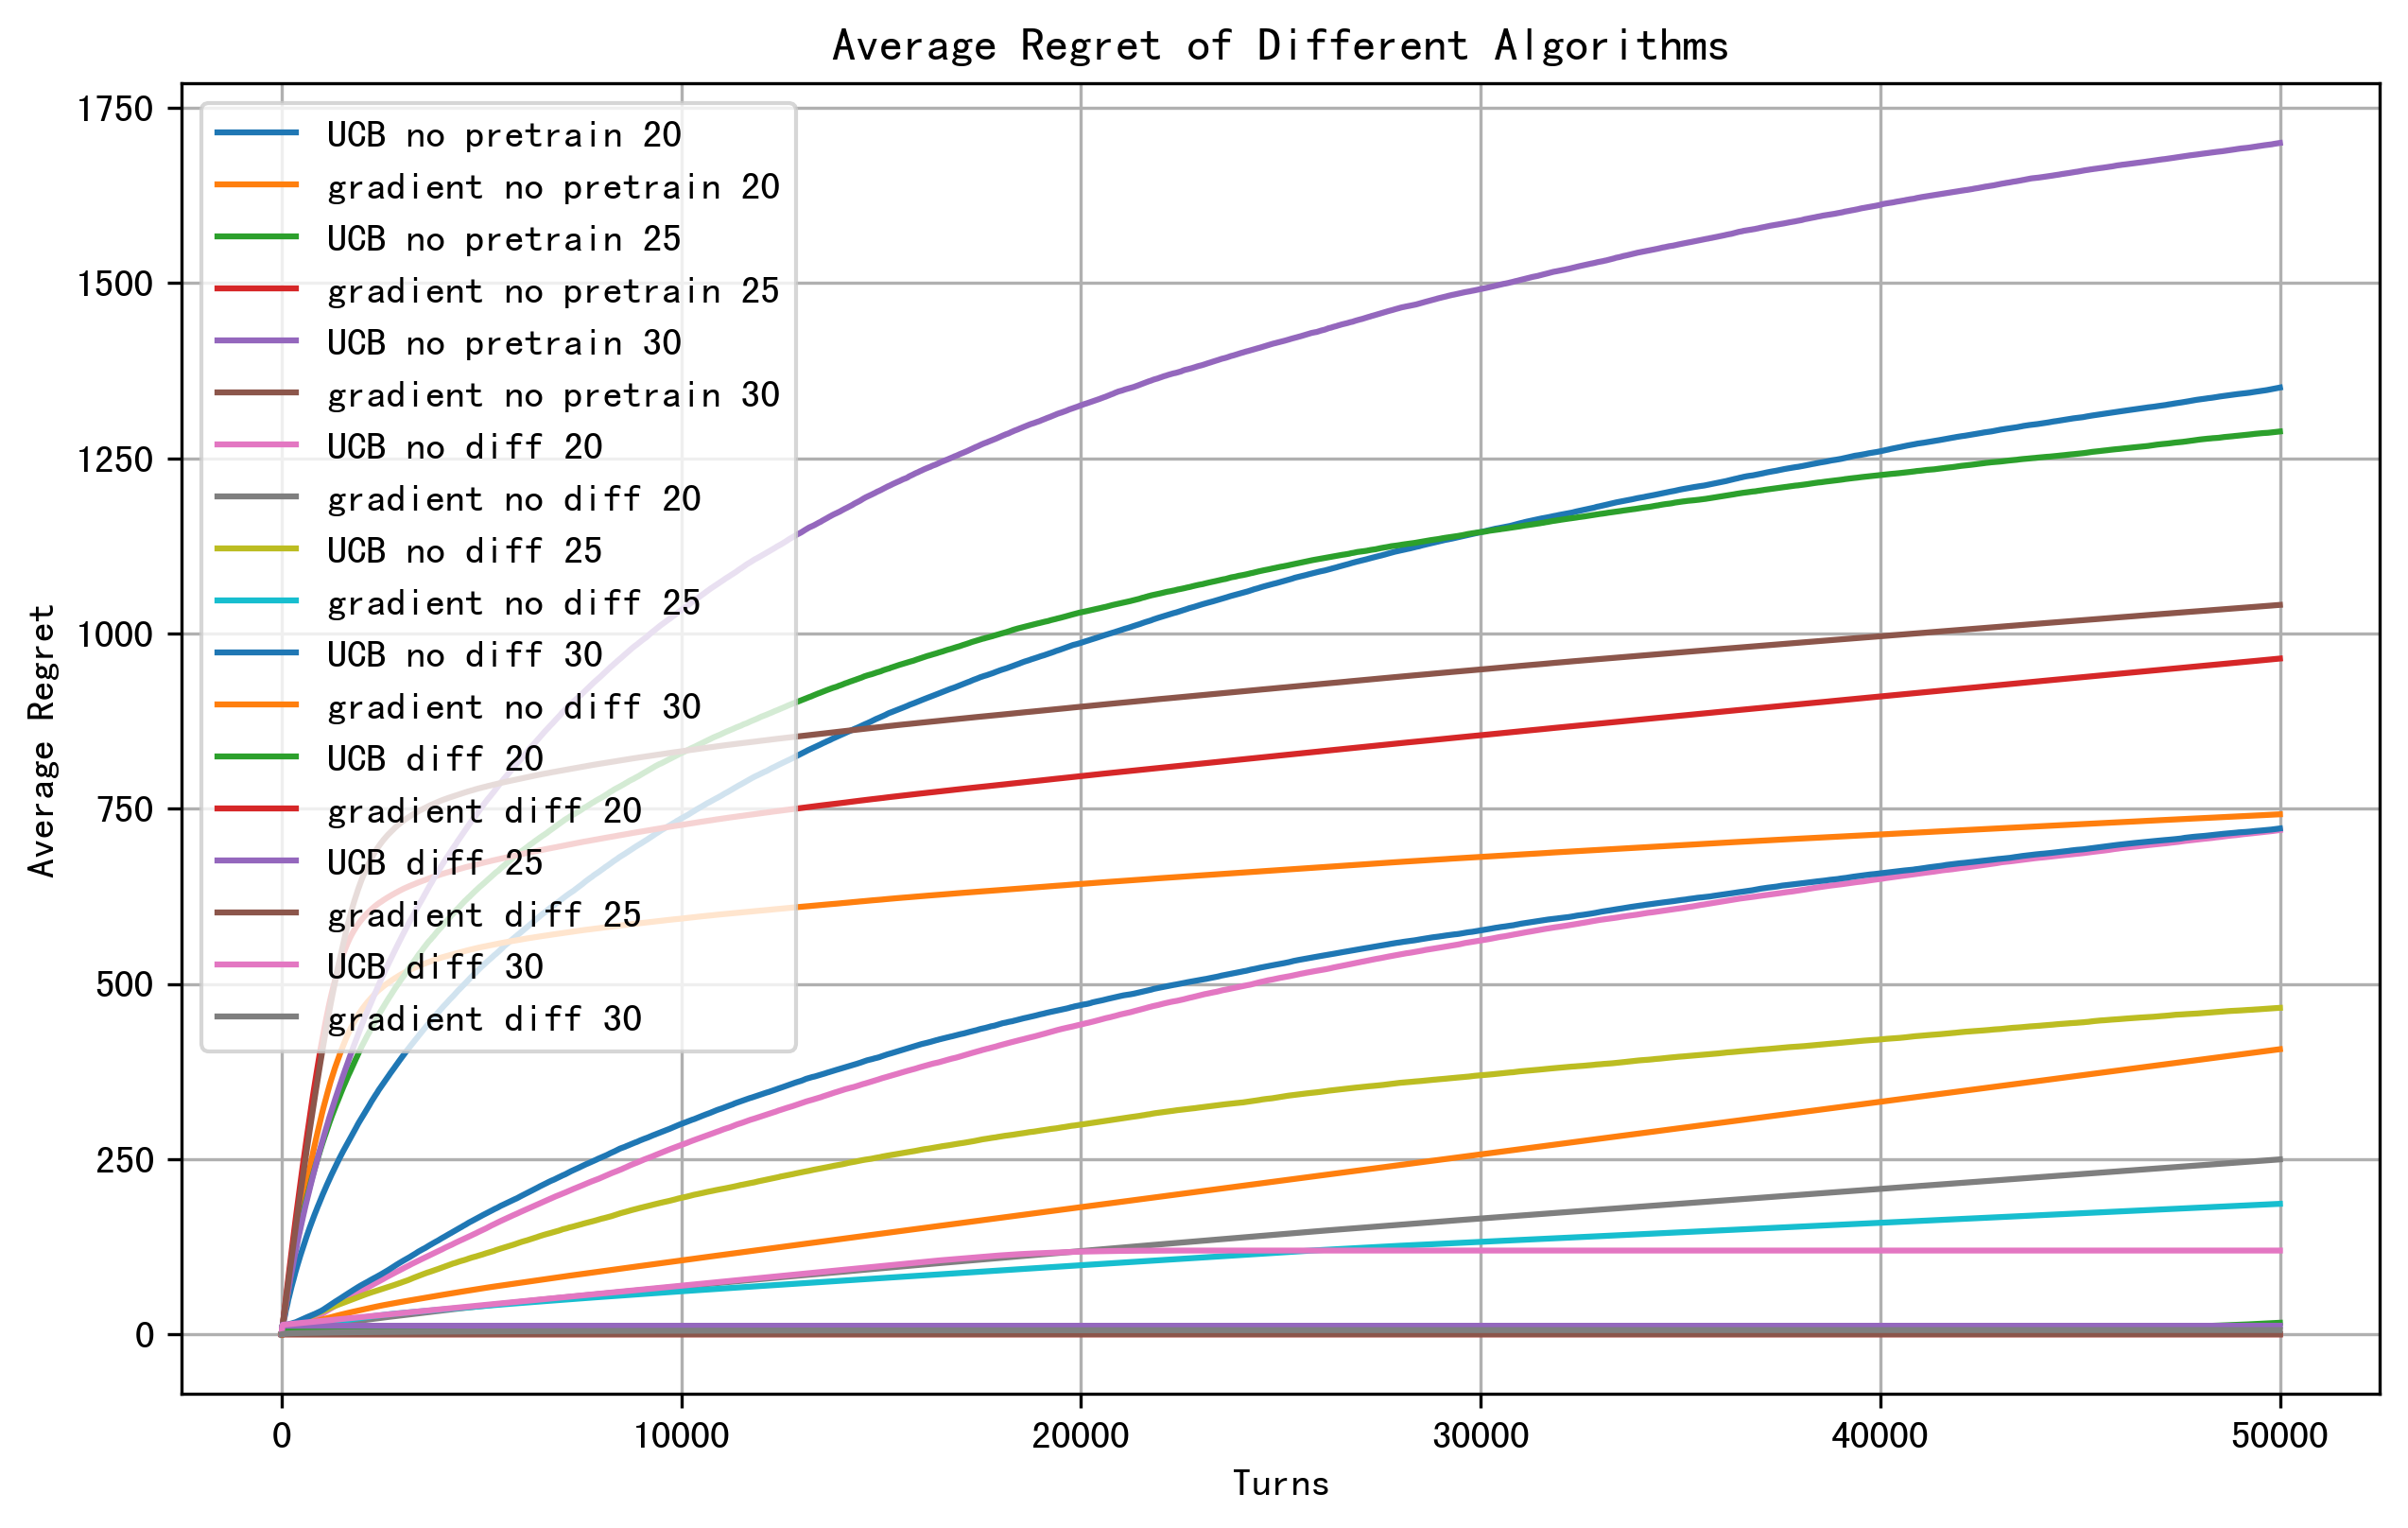
\includegraphics[width=\linewidth]{./Img/stochastic_non_bern.png}
    % \vspace{-1in}
\end{tikzfigure}
    }

   

    \column{0.32}
    \block{Contextual Bandit Results}
    {
        Diffusion can learn the conditional distribution of 0/1 rewards from MNIST and make decisions accordingly, but underperforms compared to NeuralTS and Neural Epsilon-Greedy.
\begin{itemize}
    \item The aleatoric uncertainty learned in Diffusion is unnecessary for Bernoulli-type rewards, and instead increases the randomness of its outcomes.
    \item Its advantage in modeling complex distributions (e.g., multimodal, heavy-tailed) is less relevant for simple binary rewards. Mean estimation suffices.
\end{itemize}
        
\begin{tikzfigure}[Comparison of cumulative regret across different algorithms after 25 rounds of pertaining using MNIST Dataset.]
    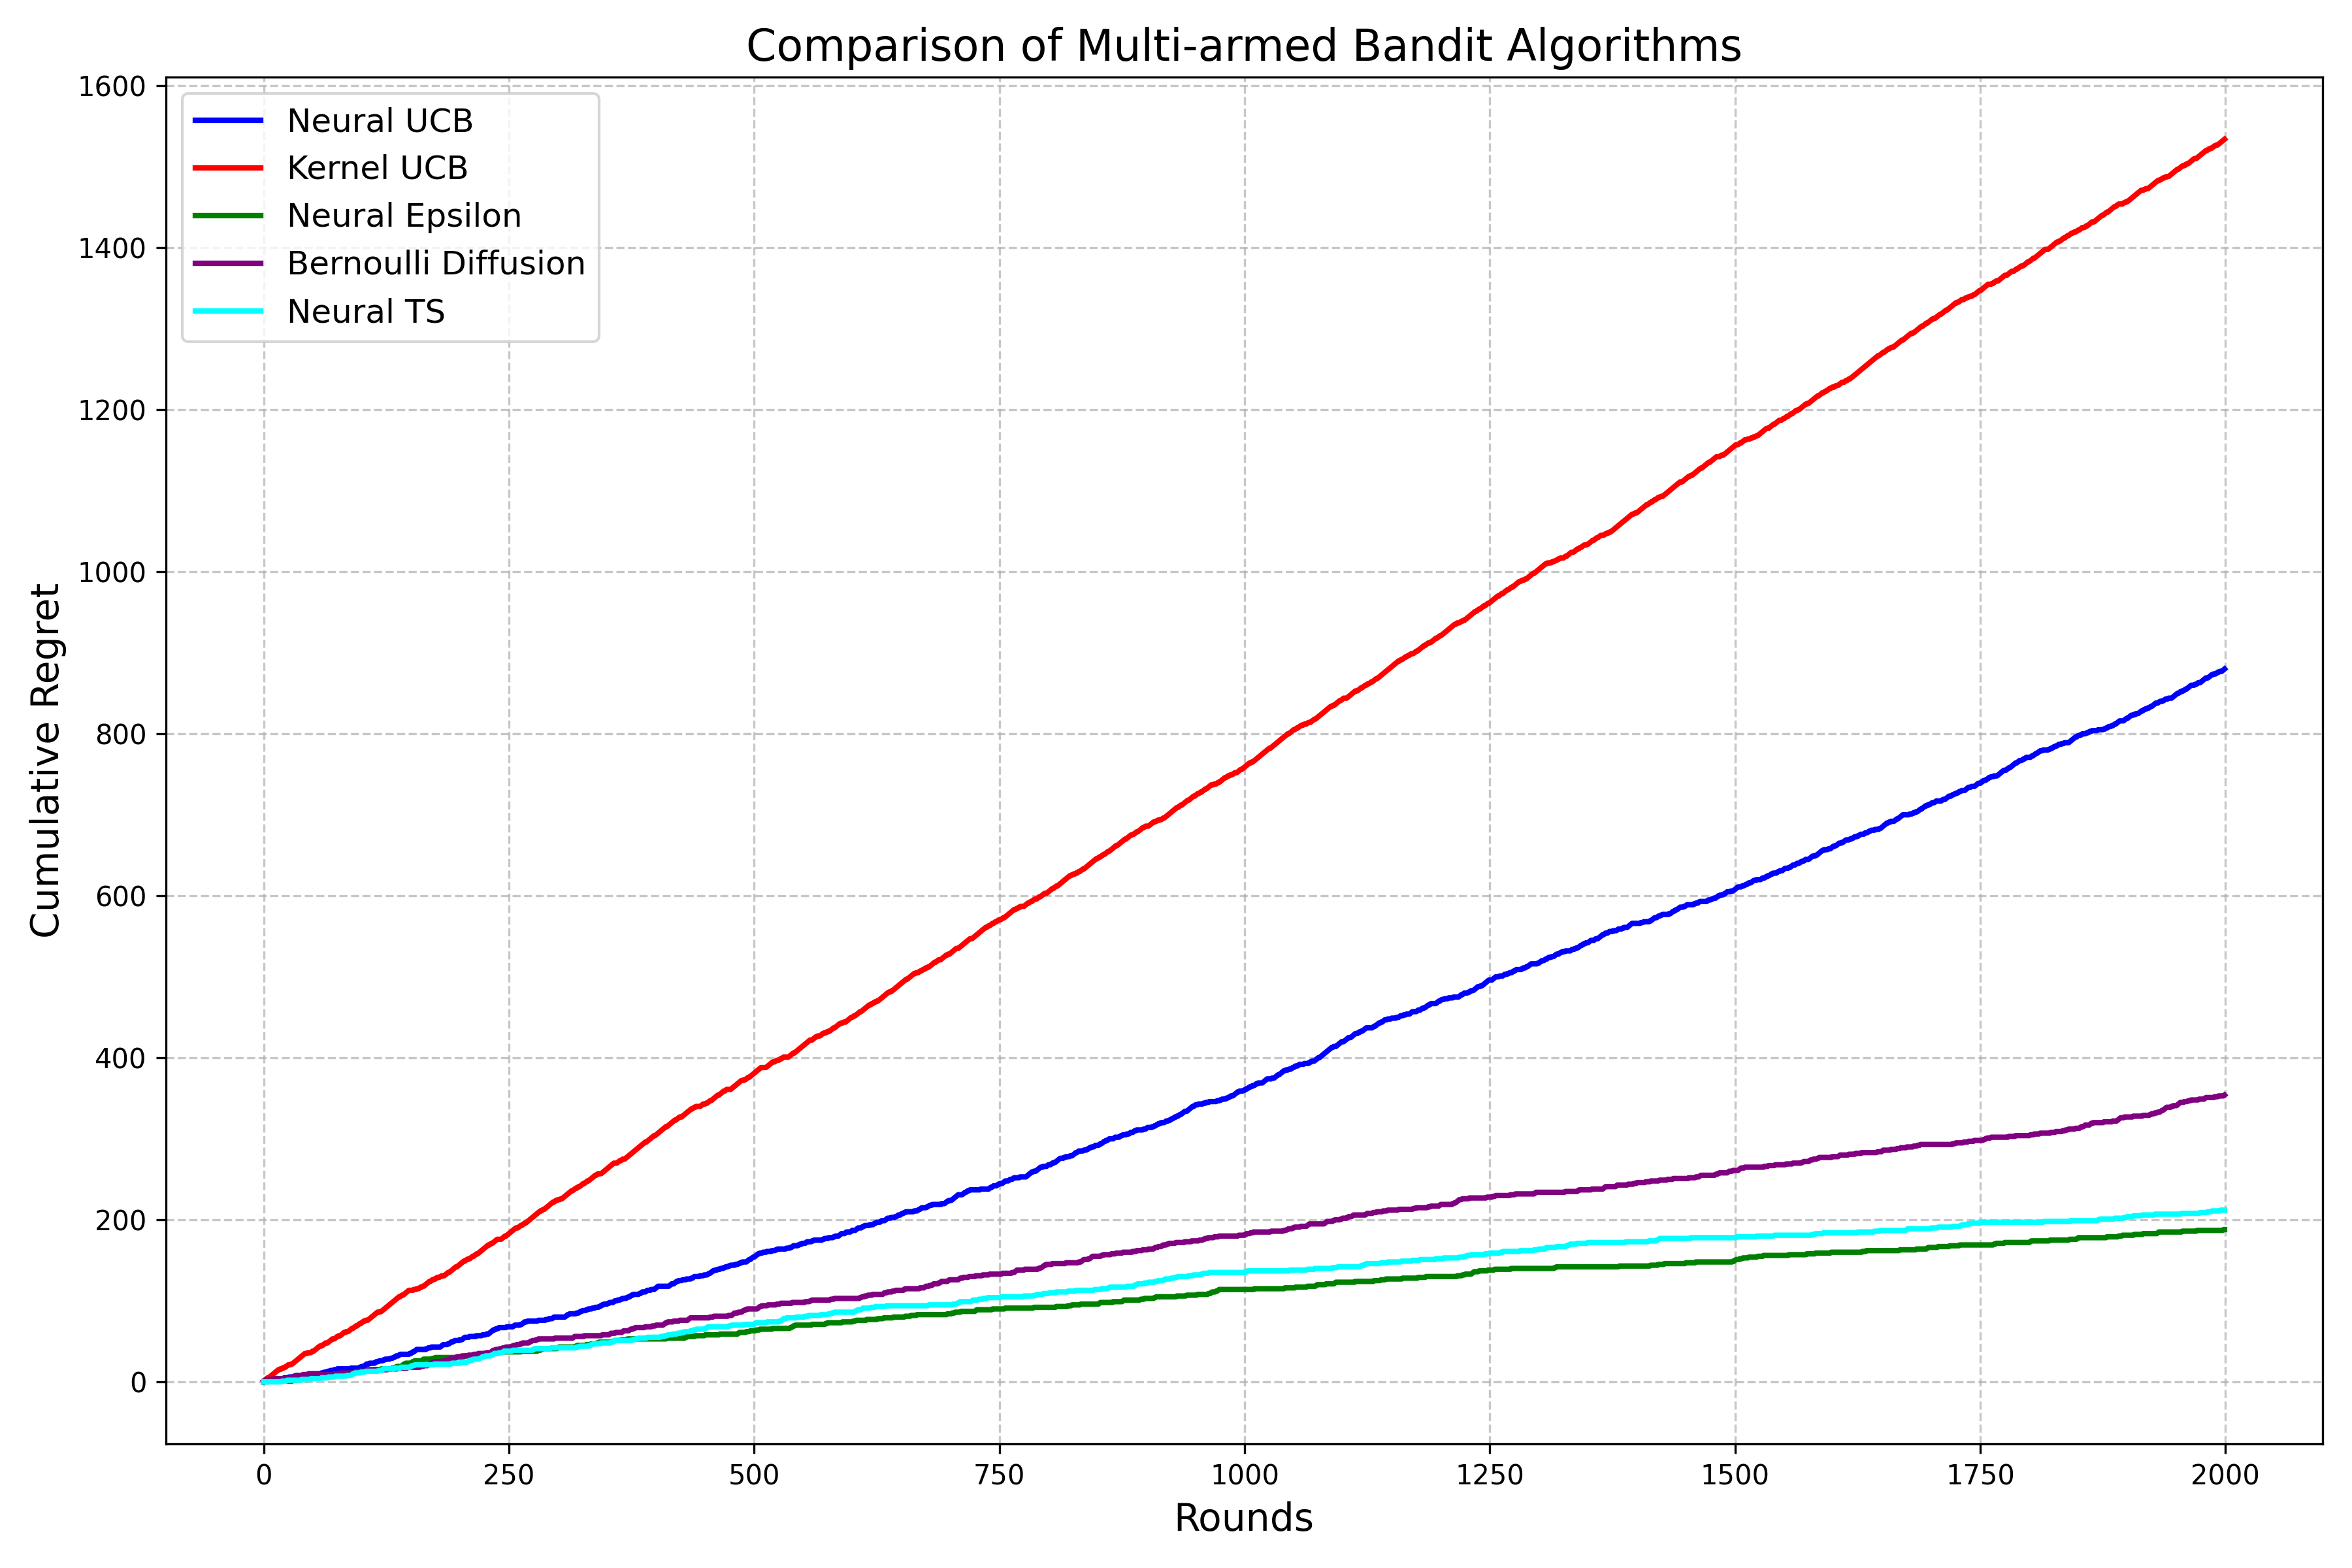
\includegraphics[width=\linewidth]{Img/context_compare.png}
\end{tikzfigure}
    }
    
    \block{Future Work}
    {
        Stochastic Bandit:
\begin{itemize}
  \item Replace the linear preference function $H_{\theta}(a)$ with kernel methods or neural networks to enhance model expressiveness and policy flexibility.
  \item Combine the discrete diffusion process with Transformer-style autoregressive generation to further improve trajectory quality.
  \item Extend the discrete diffusion model to dynamic settings such as Restless Bandits, evaluating its effectiveness in more complex decision scenarios.
\end{itemize}


Contextual Bandit:
\begin{itemize}
    \item Integrating Bayesian principles (such as Bayesian diffusion models or model ensembling) into Diffusion to more effectively quantify and leverage epistemic uncertainty (exploration).
    
    \item Additionally, exploring more sophisticated risk-sensitive decision-making rules based on the full return distribution learned by Diffusion will also be a promising direction.
\end{itemize}
    }
    \block{References}{
        \vspace{-1em}
        \begin{footnotesize}
        \printbibliography[heading=none]
        \end{footnotesize}
    }
\end{columns}
\end{document}